\chapter{Vyhodnotenie Extended Nagappan-Vouk}
Navrhnutý algoritmus adresuje nedostatky už existujúch algoritmov a odstraňuje ich, ale aby bol skutočne použiteľný je potrebné, aby všeobecne dosahoval presné výsledky a  zvládal pracovať aj z vačším množstvom dát. Ďalej nás bude zaujímať, či vieme ešte viac spresniť jeho výsledky predspracovaním logovacích správ a ako takýto preprocesing ovplyvní výkonnosť algoritmu. Ďalej preto budeme skúmať tieto otázky:

\begin{enumerate}
  \item Aká je presnosť algoritmu Extended Nagappan-Vouk na reálnych dátach ?
  \item Ako rýchlo beží algoritmus na netriviálne veľkej množine vstupných správ ?
  \item Vieme zlepšiť presnosť algoritmu predspracovaním vstupných správ ? Ovplyvní to výkonnosť algoritmu ?
\end{enumerate}

Ako základ pre naše vyhodnotenie sme použili štúdiu \parencite{he2016}. Autori v nej nazbierali dáta z piatich produkčných systémov. Tieto dáta manuálne spracovali a vytvorili tzv. golden standard, čiže ideálne rozdelenie správ na clustre. Voči tomuto rozdeleniu potom počítame hodnotu štatistiky F-measure na výsledkoch algoritmu \parencite{goldenstandard}. My sme ďalej pre každý tento dataset určili hodnoty oddeľovačov slov a dáta sme detailnejšie očistili.

\subsection{Presnosť Extendedd Nagappan-Vouk}
Ako môžme vidieť na obrázku \ref{fig:chart-precision-eng}, algoritmus pre všetky hodnoty q-percentilu dosahuje vysoké hodnoty F-Measure. Výnimkou je len dataset BGL, pre ktorý je hodnota F-Measure globálne nížšia.

	\begin{figure}[htbp]
	 \centering
	 \begin{minipage}[b]{\linewidth} 
	 	\centering	
	 	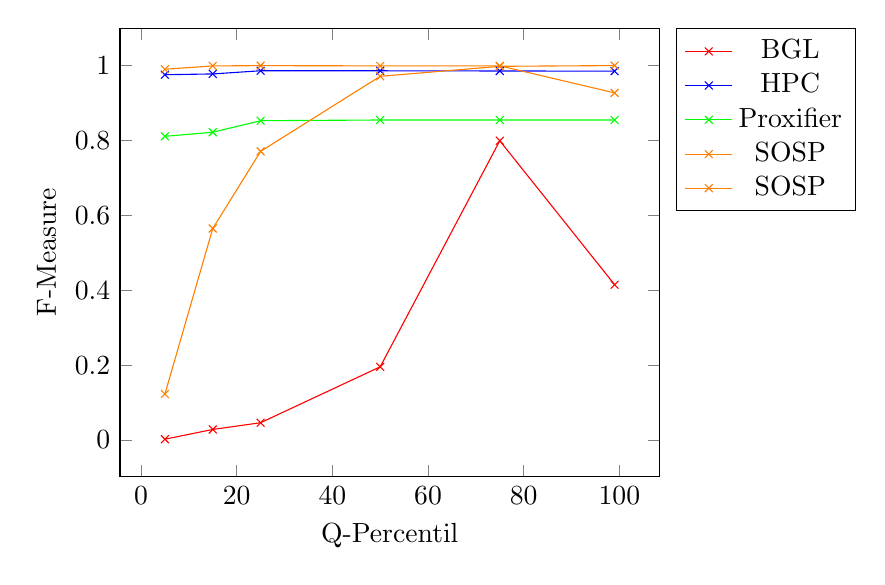
\begin{tikzpicture}
		\begin{axis}[
	    xlabel = Q-Percentil,
	    ylabel = {F-Measure},
	    legend pos=outer north east
	]
	\addplot [
	    domain=1:100, 
	    mark=x,
	    color=red,
	]
	coordinates {(5,0.0023) (15, 0.0283)  (25,0.0463) (50, 0.1956) (75, 0.7993) (99, 0.4149)};
	\addlegendentry{BGL};
	
	\addplot [
	    domain=1:100, 
	    mark=x,
	    color=blue,
	]
	coordinates {(5,0.9756) (15, 0.9777)  (25,0.9862) (50, 0.9861) (75, 0.9856) (99, 0.9851)};
	\addlegendentry{HPC};
	
	\addplot [
	    domain=1:100, 
	    mark=x,
	    color=green,
	]
	coordinates {(5,0.8111) (15, 0.8220)  (25,0.8528) (50, 0.8547) (75, 0.8547) (99, 0.8547)};
	\addlegendentry{Proxifier};
	
	\addplot [
	    domain=1:100, 
	    mark=x,
	    color=orange,
	]
	coordinates {(5,0.1229) (15, 0.5650)  (25,0.7709) (50, 0.9713) (75, 0.9981) (99, 1.0000)};
	\addlegendentry{SOSP};
	
	\addplot [
	    domain=1:100, 
	    mark=x,
	    color=orange,
	]
	coordinates {(5,0.9903) (15,0.9991)  (25,0.9999) (50, 0.9992) (75, 0.9993) (99, 0.9271)};
	\addlegendentry{SOSP};
	 
		\end{axis}
	\end{tikzpicture}
 	\caption{Presnosť algoritmu}
 	\label{fig:chart-precision-eng}
 \end{minipage}
\end{figure} 


\subsection{Výkonnosť Extendedd Nagappan-Vouk}
Uznávame, že dané datasety o mohutnosti 2000 záznamom nie sú dostačujúce na vyvodenie záveru, ale poskytujú základný prehľad o výkonnosti algoritmu. Keď namerané čísla porovnáme s výsledkami z \parencite{he2016} vidíme, že Extended Nagappan-Vouk pracuje pomalšie ako SLCT alebo IPLoM, ale radovo sú časy behu rovnaké. Je potrebné si všimnúť koreláciu medzi F-Measure a dĺžkou behu algoritmu. Čím je F-Measure vyššie a analýza presnejšia, tým sa skracuje čas potrebný na spracovanie daného datasetu.

	\begin{figure}[htbp]
	 \centering
	 \begin{minipage}[b]{\linewidth} 
	 	\centering	
	 	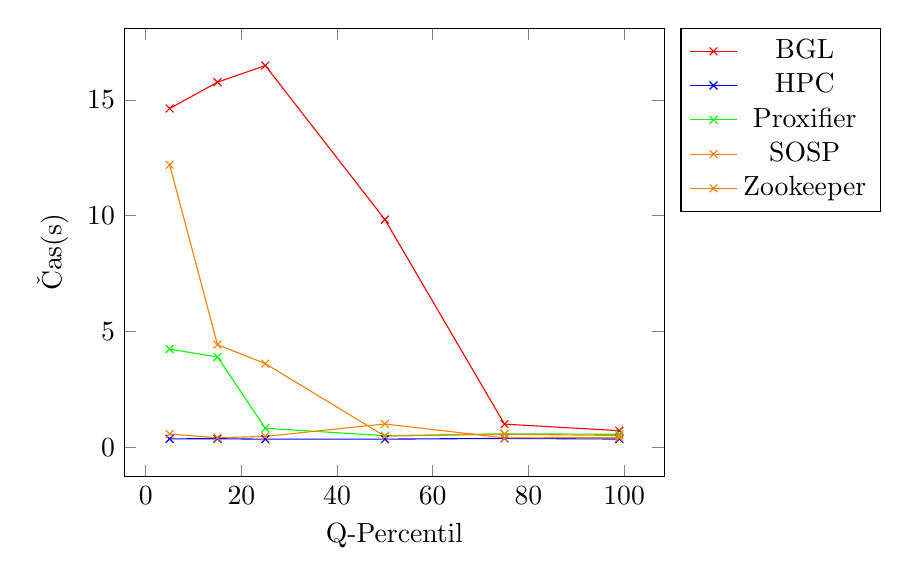
\begin{tikzpicture}
		\begin{axis}[
	    xlabel = Q-Percentil,
	    ylabel = {Čas(s)},
	    legend pos=outer north east
	]
	\addplot [
	    domain=1:100, 
	    mark=x,
	    color=red,
	]
	coordinates {(5,14.624) (15, 15.761)  (25,16.479) (50, 9.827) (75, 0.992) (99, 0.709)};
	\addlegendentry{BGL};
	
	\addplot [
	    domain=1:100, 
	    mark=x,
	    color=blue,
	]
	coordinates {(5,0.356) (15, 0.362)  (25,0.342) (50, 0.344) (75, 0.375) (99, 0.348)};
	\addlegendentry{HPC};
	
	\addplot [
	    domain=1:100, 
	    mark=x,
	    color=green,
	]
	coordinates {(5,4.232) (15, 3.895)  (25,0.814) (50, 0.492) (75,0.575) (99, 0.552)};
	\addlegendentry{Proxifier};
	
	\addplot [
	    domain=1:100, 
	    mark=x,
	    color=orange,
	]
	coordinates {(5,12.197) (15, 4.427)  (25,3.604) (50, 0.473) (75, 0.557) (99, 0.503)};
	\addlegendentry{SOSP};
	
	\addplot [
	    domain=1:100, 
	    mark=x,
	    color=orange,
	]
	coordinates {(5,0.565) (15,0.404)  (25,0.463) (50, 0.9992) (75, 0.399) (99, 0.406)};
	\addlegendentry{Zookeeper};
	 
		\end{axis}
	\end{tikzpicture}
 	\caption{Presnosť algoritmu}
 	\label{fig:chart-precision-eng}
 \end{minipage}
\end{figure} 

\subsection{Spresnenie algoritmu predspracovaním}
Zistili sme, že správne odhaliť parsovacie vzory zo správ, ktoré obsahujú parametre typu ip adresa alebo email môže byť náročné, kvôli potrebe správne nastaviť hodnotu oddeľovačov slov tak, aby boli správne rozpoznané ako jeden parameter. Preto sme chceli overiť, či dodatočné predspracovanie správ a nahradenie týchto parametrov ich hashom zmenší závislosť na správnom nastavení oddeľovačov slov a zvýši presnosť.

\par Empirickou metódou sme určili zoznam kandidátov na takúto zámenu. Sú to tieto parametre:

\begin{enumerate}
  \item Url
  \item Email
  \item Hostname
  \item Ip adresa
  \item ISO časová známka
\end{enumerate}

Pred samotnou analýzou teda prejdeme všetky správy a každý výskyt jedného z vymenovaných parametrov nahradíme jeho hashom. Pri samotnom behu algoritmu Nagappan-Vouk teda nedôjde k rozdelenie podľa oddeľovača slov. Ďalej už algorimus postupuje štandardne ako bolo popísane v \ref{sec:eng}. Porovnaním výsledkov sme zistili, že nami prezentované riešenie neviedlo k zlepšeniu presnosti parsovacích vzorov. Priemer F-Measure pôvodného algoritmu je 0.81 pričom priemer verzie s predspracovaním je len 0.78. Čísla za jednotlivé datasety ukazujú, že v prípadoch, kde pôvodný algoritmus dosiahol nízku presnosť, upravená verzia nebola schopná túto presnosť výrazne prekonať. V datasetoch s vysokou presnosťou nami upravený algoritmus len kopíruje pôvodnú verziu a pre dataset Zookeeper dokonca zhoršuje priemernú presnosť. Tieto merania sú ale špecifické tým, že parameter oddeľovačov slov je nastavený podľa znalosti domény daného datasetu a preto pôvodná verzia produkuje veľmi presné výsledky. Ďalej sme zistili, že takéto predspracovanie výkonnosť algoritmu ovplyvňuje len nepatrne.